\documentclass[a4paper]{amsart}            %for bookmarks enable option [liststotoc]%



%-------packages-------------------------%

%Languages: Uncomment for German Package:
\usepackage[latin1]{inputenc} %gives Umlauts
%\usepackage[T1]{fontenc} 
%\usepackage[ngerman]{babel} 

\usepackage{amsmath}
\usepackage{amsthm}        % Does theorem stuff
\usepackage{amssymb} 


%-------Biblatex ------------------------%

%there was however the problem, that I could not get the spacing for the headline right - depends on parskip!
\usepackage[natbib=true,style=numeric,sorting=none]{biblatex}
\bibliography{over2}
\renewcommand{\bibfont}{\normalfont\footnotesize}

%----------------------------------------%


\usepackage{tikz}
\usepackage{pgf}
\usetikzlibrary{calc, through, matrix, arrows,positioning, decorations.pathmorphing }

\usepackage[margin=1.5in]{geometry}

\usepackage{enumitem}

\usepackage{tikz}
\usetikzlibrary{%
  matrix,%
  calc,%
  arrows%
}

\usepackage{csquotes}

\usepackage{color}
\usepackage{hyperref}

\usepackage{braket}


\definecolor{darkblue}{gray}{0.25}
\definecolor{darkblue}{rgb}{0.0,0.0,0.3}  

%pdf book marks the way I like%
\hypersetup{pdftex=true, colorlinks=true, breaklinks=true, linkcolor=darkblue, menucolor=darkblue, urlcolor=darkblue}


%-----------style------------------------%

%\addtolength{\parskip}{\baselineskip} %Absätze im Text werden auch tatsächlich zu Absätzen%
\parindent 0pt

%----------new--commands-----------------%

\newcommand{\C}{\mathcal{C}}
\renewcommand{\O}{\mathcal{O}}
\newcommand{\D}{\mathcal{D}}
\newcommand{\F}{\mathcal{F}}
\newcommand{\G}{\mathcal{G}}
\newcommand{\ve}{\varepsilon}
\newcommand{\Mor}{\mathrm{Mor}}
\newcommand{\id}{\operatorname{id}}
\newcommand{\Hom}{\operatorname{Hom}}
\newcommand{\Z}{\mathbb{Z}}
\newcommand{\N}{\mathbb{N}}

% --- homology ---- %
\newcommand{\HCW}[1]{\widetilde{H}^{\operatorname{CW}}_{#1}}
\newcommand{\Hred}[1]{\widetilde{H}_{#1}}
\newcommand{\CWchain}[1]{\widetilde{C}^{\operatorname{CW}}_{#1}}
\newcommand{\dCW}[1]{d^{\operatorname{CW}}_{#1}}

\DeclareMathOperator{\coker}{coker}
\DeclareMathOperator{\im}{im}
\DeclareMathOperator{\tr}{tr}

%this is a nice way to display x mod n. Use: \imod
\makeatletter
\def\imod#1{\allowbreak\mkern10mu{\operator@font mod}\,\,#1}
\makeatother


% the following code will uplift the \maketitle title. In standard it is way too low.
\makeatletter % wegen @ in den Befehsnamen
\renewcommand*\@maketitle{%
  \normalfont\normalsize
  \@adminfootnotes
  \@mkboth{\@nx\shortauthors}{\@nx\shorttitle}%
% (SCHW) auskommentiert:  \global\topskip42\p@\relax % 5.5pc   "   "   "     "     "
  \@settitle
  \ifx\@empty\authors \else \@setauthors \fi
  \ifx\@empty\@dedicatory
  \else
    \baselineskip18\p@
    \vtop{\centering{\footnotesize\itshape\@dedicatory\@@par}%
      \global\dimen@i\prevdepth}\prevdepth\dimen@i
  \fi
  \@setabstract
  \normalsize
  \if@titlepage
    \newpage
  \else
    \dimen@34\p@ \advance\dimen@-\baselineskip
    \vskip\dimen@\relax
  \fi
} % end \@maketitle
\makeatother

%--------new--enviroments----------------%

\renewcommand{\theequation}{\thesection.\arabic{equation}}         %%                             %I somehow need this for the warning symbol to work 
 \makeatletter                                                      %%                             properly, I don't really know why though%
    \@addtoreset{equation}{section} % Make the equation counter reset each section
    \@addtoreset{footnote}{section} % Make the footnote counter reset each section
                                                                    %%
 \newenvironment{warning}[1][]{%                                    %%
    \begin{trivlist} \item[] \noindent%                             %%
    \begingroup\hangindent=2pc\hangafter=-2                         
    \clubpenalty=10000%                                             										
    \hbox to0pt{\hskip-\hangindent\manfntsymbol{127}\hfill}\ignorespaces%
    \refstepcounter{equation}\textbf{Warning~\theequation}%         
    \@ifnotempty{#1}{\the\thm@notefont \ (#1)}\textbf{.}            
    \let\p@@r=\par \def\p@r{\p@@r \hangindent=0pc} \let\par=\p@r}%  
    {\hspace*{\fill}$\lrcorner$\endgraf\endgroup\end{trivlist}}  
    
    
%\newenvironment{beweis}{\par\begingroup%
%\settowidth{\leftskip}{\emph{Proof.~}}%																											remove to use \begin{beweis}
%\noindent\llap{\emph{Proof.~}}}{\hfill$\Box$\par\endgroup}     
    
  

\newenvironment{tmo}[1]{%
  \trivlist
  \leftskip=0.15cm
  \item[\hskip\labelsep
        \bfseries
   #1\@{.}]\mbox{ }\par\nobreak
   \vskip -0.5em\nobreak% Absatzabstand nachträglich entfernen.
   \noindent
  \leftskip=0.35cm
  \rightskip=0.35cm
  \itshape\ignorespaces
}{%
\endtrivlist}

\newcounter{tm}
% Falls tm abhängig von \section nummeriert werden soll:
%\numberwithin{tm}{section}% anderenfalls auskommentieren!!!
\newenvironment{tm}[1]{% wie tmo aber mit Nummer
  \refstepcounter{tm}%
  \tmo{#1~\thetm}%
}{%
  \endtmo
}
     
\makeatletter
\renewenvironment{proof}[1][\proofname]{\par
  \pushQED{\qed}%
  \normalfont \topsep6\p@\@plus6\p@\relax
  \trivlist
  \leftskip=0.6cm
  
  \item[\hskip\labelsep
        \itshape
    #1\@addpunct{.}]\mbox{ }\par\noindent%
  \leftskip=1cm
  \rightskip=1cm    
}{%
  \popQED\endtrivlist\@endpefalse
}
\makeatother 

\theoremstyle{plain}                                               %%
 \newtheorem{theorem}[equation]{Theorem}                            %%
 \newtheorem*{claim}{Claim}                                         %%
 \newtheorem*{lemma*}{Lemma}
 \newtheorem*{proposition*}{Proposition}                                       %%
 \newtheorem*{theorem*}{Theorem}                                    %%
 \newtheorem{lemma}[equation]{Lemma}                                %%
 \newtheorem{corollary}[equation]{Corollary}                        %%
 \newtheorem{proposition}[equation]{Proposition}                    %%

%--produce-the-warning--symbol-----------%
 \DeclareFontFamily{U}{manual}{}                                
 \DeclareFontShape{U}{manual}{m}{n}{ <->  manfnt }{}            
 \newcommand{\manfntsymbol}[1]{%                                
    {\fontencoding{U}\fontfamily{manual}\selectfont\symbol{#1}}}

\makeatother


\begin{document}

%------------header----------------------%

\title{An Outline of Quantum Mechanics}
%\author{Felix Hoffmann}% %for now I decided against it%


\maketitle
\pagestyle{empty} %no pagenumbers and titles%
\thispagestyle{empty}

\abovedisplayskip\bigskipamount
\belowdisplayskip \abovedisplayskip
\parskip 12pt plus 1pt minus 1pt

%-------end header-----------------------%

Quantum mechanics is, viewed purely as a mathematical theory, a generalisation of probability theory (a \emph{non-commutative} probability theory). Application to a concrete problem however, reduces the theory to a probability theory in the classical sense \mbox{\cite[p. 280]{qp}}. Quantum Mechanics thus (only) aspires to yield expectation values and probability distributions for the outcomes of statistical experiments. 

In such an experiment, two phases that may be distinguished: \textbf{Preparation} and \textbf{measurement}. This separation comes naturally, the two processes are essentially independent: The same measurement procedure may be used on differently prepared particles, as much as different measurements may be performed on identically prepared particles.

\bigskip



\begin{center}
\hspace{+0.5cm}
\resizebox{11.5cm}{!}{%
	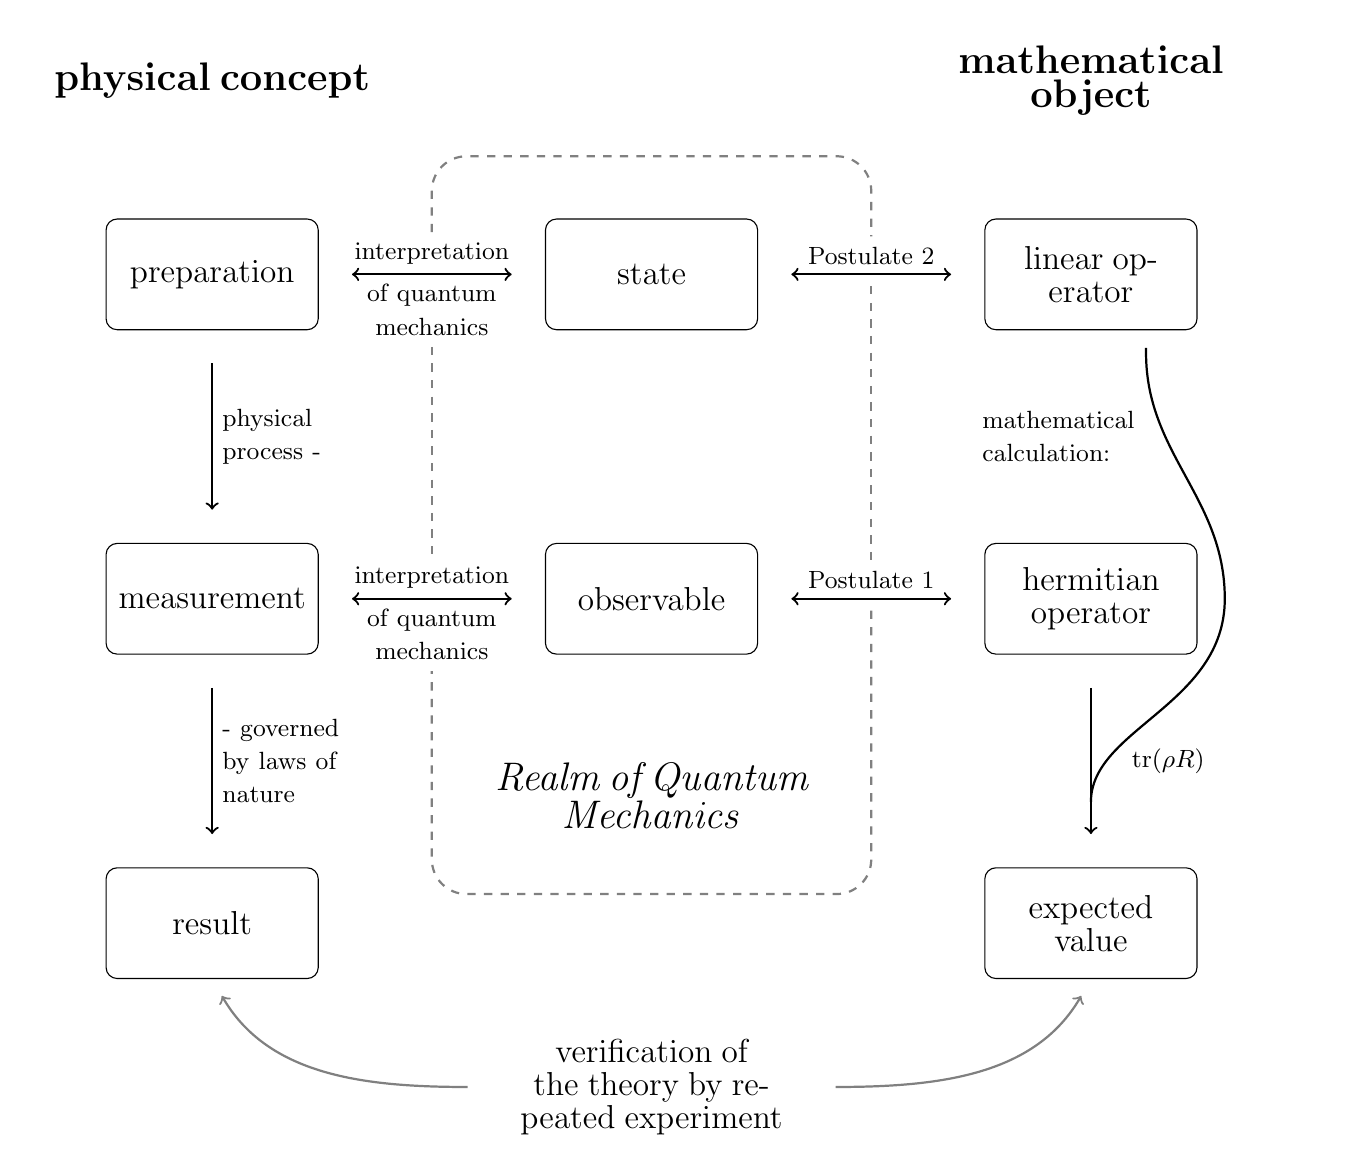
\begin{tikzpicture}[auto]
	\tikzstyle{equi} = [<->,draw, thick, shorten <=12pt, shorten >=12pt];
	\tikzstyle{to} = [->,draw, thick, shorten <=12pt, shorten >=12pt];
	\tikzstyle{block} = [rectangle, draw, text width=7em, text centered, rounded corners, minimum height=4em]    
	\tikzstyle{head} = [rectangle,  text width=12em, text centered, rounded corners]
	
	\matrix [column sep=20mm,row sep=27mm,ampersand replacement=\&]
	{
		% row 0
			\node [head]  				(pc)					{\Large \textbf{physical concept}}; \&
								\&
			\node [head] 					(mc)					{\Large \textbf{mathematical object}}; \\[-15mm]	
		% row 1
			\node [block]  				(prep)				{\large preparation}; \&
			\node [block] 				(state)				{\large state}; \&
			\node [block] 				(linop)				{\large linear operator}; \\
		% row 2
			\node [block]					(meass) 			{\large measurement}; \& 
			\node [block]					(observable) 	{\large observable}; \& 
			\node [block]					(hermop)			{\large hermitian operator}; \\																							
		% row 3
			\node	[block]		(result)			{\large result};\&		
																			 \&
			\node [block]		(eval) 				{\large expected value}; \\
	};
	
	\node[above of=state, node distance = 1.5 cm] (upper mid) {};
	\node[below of=observable, node distance = 3.75 cm] (lower mid) {};
	\node[below of=observable, node distance = 2.50cm, text width=5cm, text centered] {\Large \emph{Realm of \mbox{Quantum} Mechanics}};
	\node[right of=hermop, node distance = 1.7 cm] (hermop right) {};
	\node[right of=linop, node distance = 0.7cm] (linop right) {};

	
	%horizontal paths
	\tikzstyle{every path}=[equi]
	
		\path (prep) -- node (upper left) {\small interpretation} node[below,text width=2cm, text centered] {\small of quantum mechanics} (state) ;
		\path (meass) -- node[above] (lower left) {\small interpretation} node[below,text width=2cm, text centered] {\small of quantum mechanics} (observable);
		\path (state) -- node (upper right) {\small Postulate 2} (linop);
		\path (observable) -- node (lower right) {\small Postulate 1} node[below=90pt] (lowri) {} (hermop);
		

	
	%vertical paths
	\tikzstyle{every path}=[to]
		
		\path (hermop) -- node(hermop-eval){}(eval);
		\path (prep) -- node[text width=1.5cm] (prepmess) {\small physical process -} (meass);
		
\node[below of=hermop, node distance=3cm]  (hermoplow) {};
		\path [draw,-,shorten <=23pt] (linop right) -- +(0,-1) to [out=270,in=90](hermop right.center) to [out=270,in=90] (hermoplow.center);
		\path (meass) -- node (messre)[text width=2cm] {\small - governed by laws of nature} (result);
		
\node[right of=prepmess, node distance = 9.9cm, text width = 2cm] {\small mathematical calculation:};
\node[right of=messre, node distance = 11.8cm, text width= 2.5cm] {\small $\tr(\rho R)$};
\node[below=4.75cm of observable, text width = 4.2cm, text centered] (verif) {\large verification of the theory by repeated experiment};

\tikzstyle{every path}=[draw, gray, ->, shorten >=7pt, shorten <= 3pt, thick]
	\path (verif.east)  to 	[out=0,in=240] 			(eval.south);
	\path (verif.west) 	to 	[out=180, in=300] 	(result.south);
	
	
	%\draw[dashed, rounded corners=10pt] (upper left)+(0,1.2) rectangle (lowri);
	\tikzstyle{every path}=[draw, thick, dashed, rounded corners=12.5pt, gray]
		\path (upper left) 	|- 	(upper mid.center) 	-| 	(upper right);
		\path (upper right) -- 	(lower right) [shorten <=0.15cm];
		\path (lower right) |- 	(lower mid.center) [shorten <=0.15cm] - |  (lower left) [shorten >=0.92cm];
		\path (upper left) 	-- 	(lower left) [shorten <=0.92cm];
	
	
	\end{tikzpicture}
}
\end{center}
   
\bigskip

The quantum mechanical concept connected to measurement is that of an \textbf{observable}. Since not all abstract quantities inherent to the system might be measurable (the trajectory of an electron is such an example), one declares as an observable only those variables of a system that can in principle be measured \cite{OpAlg}.

In a classical theory, the range of possible values for such a variable is commonly assumed to be continuous. Considering the energy levels of electrons in atoms however, we know that a proper quantum theory also needs to account for a discrete spectrum of possible values of measurement. 

\textbf{Postulate 1}: \itshape The mathematical object assigned to the physical observable shall be a linear operator. It's spectrum shall reflect the possible values of the dynamical variable. \upshape

This makes sense in so far that there are linear operators that have a continuous spectrum and there are such that have a discrete spectrum. 

The concept tied to preparation is that of a \textbf{state}. The preparation determines the probability distribution for the outcomes of a following measurement. In fact, it is \emph{independent} of the measurement and necessarily determines the probabilities for \emph{any} subsequent measurement. We identify the state with the specification of a probability distribution for every observable.

\textbf{Postulate 2}: \itshape To each state corresponds a unique linear operator $\rho$ with $\tr(\rho)=1$. The expected value for the observable $R$ in the state $\rho$ is given by \upshape 
\[\tr(\rho R).\]

Given a physical experiment, we are able to translate it into the realm of quantum mechanics by selecting a state, representing the preparation procedure, and an observable, representing the measurement procedure. Postulates 1 and 2 then correspond these quantum mechanical concepts to mathematical objects. The postulates, however, yield more than just this identification, in the mathematical realm we obtain a \emph{probability theory}. This result is known as the \emph{spectral theorem} and has seen numerous proofs \mbox{\cite{OpAlg,reedsimon}}. 

Using this theory, we write the observable $R$ as \[R=\int \lambda\, dE_R(\lambda),\] where the map $E_R(\cdot)$, which assigns a linear operator to every measurable subset of $\mathbb{R}$, is called the \emph{projection valued measure} of $R$.  Then the probability of the measurement outcome lying in an interval $B$ of $\mathbb{R}$, for a system prepared in the state $\rho$, is given by \[\operatorname{Pr}(B)=\tr(\rho\, E_R(B)).\] 

Having transfered the physical experiment to a probability theory, we are now able to test our quantum theory by repeating the experiment and comparing the results with the expected values, calculated from by the probability theory. 

It should be noted, that, while we utilize the intricate connection between probability and frequency to verify our theory, the frequentist view on probability \cite{stanford} might not be too helpful when trying for an interpretation of quantum mechanics. Leslie Ballentine advises to adopt the propensity interpretation instead \cite[p. 32]{Ballentine_2003}, while John Baez suggests that the Bayesian interpretation might be preferable \cite{Baez}.

The two postulates given are, however, not sufficient to account for all aspects of quantum mechanics. As opposed to the classical case, measurement in quantum mechanics strongly influences the outcomes of subsequent measurements. The principle of \emph{state reduction} has been axiomatized by von Neumann \cite{neumann}:

\newpage
\textbf{Postulate 3}: \itshape After obtaining eigenvalue $r$ of the observable $R$ as a result of measurement of a system prepared in the state $\rho$, the new state of the system is given by \[\rho' = \frac{P_r\,\rho\,P_r}{\tr(P_r\,\rho)},\]  where $P_r$ is the projection operator onto the eigenspace of $r$.   \upshape

\vspace{0.47cm}
\section*{\textbf{Dynamics}}

So far we didn't really do justice to the \enquote{mechanics-part} in quantum mechanics. Dynamics enter the picture, when we look at the time evolution of a given system. As the corresponding states and observables already completely determine the (quantum mechanical) behaviour of this system, only a time evolution of those can account for dynamical properties. In the \emph{Schrödinger picture} the states evolve in time, in the \emph{Heisenberg picture}, it is the observables that depend on a time parameter. Whether time dependence of observables or states is causing dynamics is only philosophically interesting at best, mathematically the formulations are shown to be equivalent.

Time evolution in either case is implemented by a \emph{time evolution operator} $U(t,t_0)$. The operator should evolve states $\rho$ via
\[
\rho(t) = U^{\dagger}(t,t_0)\, \rho(t_0)\, U(t,t_0),
\]
and do this continuously so. Furthermore, to guarantee probability conversation, U needs to be unitary. Is $H$ the Hamilton operator for a given system, the time evolution operator satisfies
\vspace{0.4cm}
\[
i\hbar \partial_t U(t,t_0) = H U(t,t_0),
\]

the \emph{Schrödinger equation}. At this point quantum mechanics stops being a purely mathematical formulation and becomes a proper physical theory: to obtain results that can be verified by experiment, the Hamiltonian $H$ must be chosen in such a way, that it represents the given physical system. 

\bigskip
\bigskip
\bigskip
\bigskip
\parskip 5pt
\printbibliography

\end{document}
